\chapter{Teoria del propagatore}
Adesso che si sono quantizzati i campi scalari e spinoriali ad un istante di temo $t$ fissato ed si sono interpretati i risultati ottenuti in termini di particelle relativistiche, si vuole ora studiare l'evoluzione temporale di tali campi. Il concetto fondamentale per questo scopo è quello di propagatore la cui espressione esplicita funge da base per i diagrammi di Feynman e il calcolo delle sezioni d'urto dei processi di scattering tra particelle relativistiche. In Teoria dei campi, il propagatore non fornisce altro che l'ampiezza di probabilità che una particella viaggi da un luogo ad un altro in un dato tempo, ovvero anche con una certa energia e momento. Anche se potrebbe sembrare, il concetto di propagatore non è niente di nuovo: in Meccanica quantistica non relativistica il propagatore fornisce infatti la probabilità che una particella che si trova in un punto $\vx_i$ dello spazio al tempo $t_i$, arrivi in un altro punto $\vx_f$ al tempo $t_f$ ed è definito come l'elemento di matrice 
\begin{equation}
\label{eq: propagatore in MQ non relativistica}
    K(\vx_i,t_i;\vx_f,t_f) = \mybrakett{\vx_f}{\hatU(t_f,t_i)}{\vx_i}.
\end{equation}
Il propagatore può essere visto come l'inverso dell'operatore d'onda appropriato per la particella e per questo è spesso identificato con la funzione di Green di tale operatore. Infatti, il propagatore \eqref{eq: propagatore in MQ non relativistica} è la funzione di Green dell'operatore di Schr\"odinger 
\begin{equation}
    \bigg(i\frac{\p}{\p t} - \hatH\bigg)K(\vx_i,t_i;\vx_f,t_f) = -i\delta^3(\vx_f - \vx_i)\delta(t_f - t_i).
\end{equation}
Per studiare l'evoluzione temporale si è soliti usare la rappresentazione di Heisenberg per gli operatori di campo quantistici.

In generale, considerando operatori di campo $\hat{\xi}$ di qualsiasi natura, per una teoria libera, ossia prova di interazione tra i campi, il propagatore viene definito come l'elemento di matrice
\begin{equation}
\label{eq: propagatore libero generale incompleto}
    \mybrakett{0}{\hat{\xi}(x)\hat{\xi}(y)}{0},
\end{equation}
dove lo stato fondamentale è appunto lo stato di vuoto $\sv$. Tuttavia, per una teoria interagente non è più vero che lo stato fondamentale è lo stato di vuoto, invece è uno stato coincidente con una sovrapposizione infinita di autostati dell'impulso convenzionalmente indicato con $\ket{\Omega}$, che contiene, tra gli altri, anche lo stato di vuoto $\sv$. Quindi, per una teoria interagente il propagatore è definito come
\begin{equation}
\label{eq: propagatore interagente generale incompleto}
    \mybrakett{\Omega}{\hat{\xi}(x)\hat{\xi}(y)}{\Omega}.
\end{equation}
Tuttavia, queste definizioni di propagatore non sono del tutto complete: manca il contributo di antiparticella e non rispettano la causalità. Le definizioni \eqref{eq: propagatore libero generale incompleto} e \eqref{eq: propagatore interagente generale incompleto} infatti hanno senso solamente se $x^0 > y^0$, ma non comprendono il caso in cui $y^0 > x^0$, pertanto la definizione di propagatore libero completa risulta essere
\begin{equation}
\label{eq: propagatore libero generale}
    \mybrakett{0}{\hat{\xi}(x)\hat{\xi}(y)}{0}\Theta(x^0 - y^0) + \mybrakett{0}{\hat{\xi}(y)\hat{\xi}(x)}{0}\Theta(y^0 - x^0).
\end{equation}
ed analogamente quella di propagatore interagente è
\begin{equation}
\label{eq: propagatore interagente generale}
    \mybrakett{\Omega}{\hat{\xi}(x)\hat{\xi}(y)}{\Omega}\Theta(x^0 - y^0) + \mybrakett{\Omega}{\hat{\xi}(y)\hat{\xi}(x)}{\Omega}\Theta(y^0 - x^0)
\end{equation}
Le definizioni \eqref{eq: propagatore libero generale} e \eqref{eq: propagatore interagente generale} possono essere riscritte in maniera più compatta introducendo l'operatore di ordinamento temporale $T$ agente come
\begin{equation}
\label{eq: ordinamento temporale}
    T[\hat{\xi}(x)\hat{\xi}(y)] = 
    \begin{cases}
        \hat{\xi}(x)\hat{\xi}(y),\quad x^0 > y^0 \\
        \pm\hat{\xi}(y)\hat{\xi}(x),\quad y^0 > x^0
    \end{cases},
\end{equation}
dove la scelta del segno nel caso in cui $y^0 > x^0$ dipende dalla natura dei campi in questione: se si tratta di campi bosonici si sceglie il segno positivo per rispettare la simmetria, mentre se si tratta di campi fermionici si sceglie il segno meno per rispettare l'antisimmetria. Con questo operatore le espressioni dei propagatori diventano
\begin{equation}
    \mybrakett{0}{T[\hat{\xi}(x)\hat{\xi}(y)]}{0},\quad \mybrakett{\Omega}{T[\hat{\xi}(x)\hat{\xi}(y)]}{\Omega}.
\end{equation}

\section{Campo scalare carico}
In rappresentazione di Heisenberg gli operatori di campo, come visto in \eqref{eq: campo scalare carico quantizzato}, sono 
\begin{align}
    \hatphi(x) &= \int\frac{d^3k}{(2\pi)^{3/2}}\frac{1}{(2\omega_k)^{1/2}}(\hata_k e^{-ik_\mu x^\mu} + b^\dg_k e^{ik_\mu x^\mu}), \\
    \hatphid(x) &= \int\frac{d^3k}{(2\pi)^{3/2}}\frac{1}{(2\omega_k)^{1/2}}(\hataT_k e^{ik_\mu x^\mu} + b_k e^{-ik_\mu x^\mu}).
\end{align}
L'obiettivo è determinare l'espressione esplicita del propagatore 
\begin{equation}
    \Delta(x,y) = \mybrakett{0}{T[\hatphi(x)\hatphid(y)]}{0},
\end{equation}
per farlo si parte calcolando i contributi data dall'azione dei campi sullo stato vuoto. Quindi, si hanno
\begin{equation}
    \begin{split}
        \hatphid(y)\sv &= \int\frac{d^3k}{(2\pi)^{3/2}}\frac{1}{(2\omega_k)^{1/2}}(\hataT_k\sv e^{ik_\mu x^\mu} + b_k\sv e^{-ik_\mu x^\mu}) \\
        &= \int\frac{d^3k}{(2\pi)^{3/2}}\frac{1}{(2\omega_k)^{1/2}}\ket{k} e^{ik_\mu x^\mu},
    \end{split}
\end{equation}
\begin{equation}
    \begin{split}
        \bra{0}\hatphi(x) &= \int\frac{d^3k'}{(2\pi)^{3/2}}\frac{1}{(2\omega_{k'})^{1/2}}(\bra{0}\hata_{k'} e^{-ik'_\mu x^\mu} + \bra{0}b^\dg_{k'} e^{ik'_\mu x^\mu}) \\
        &= \int\frac{d^3k'}{(2\pi)^{3/2}}\frac{1}{(2\omega_{k'})^{1/2}}\bra{k'} e^{-ik'_\mu x^\mu},
    \end{split}
\end{equation}
per cui il primo contributo al propagatore libero è dato da
\begin{equation}
    \begin{split}
        \mybrakett{0}{\hatphi(x)\hatphid(y)}{0} &= \iint\frac{d^3k\,d^3k'}{(2\pi)^3(2\omega_k)^{1/2}(2\omega_{k'})^{1/2}}\mybraket{k'}{k} e^{-i(k'_\mu x^\mu - k_\mu x^\mu)} \\
        &= \int\frac{d^3k}{(2\pi)^3}\frac{1}{(2\omega_k)}e^{-ik_\mu(x^\mu - y^\mu)}.
    \end{split}
\end{equation}
Analogamente, con un simile calcolo si può arrivare al contributo di antiparticella al propagatore
\begin{equation}
    \mybrakett{0}{\hatphid(y)\hatphi(x)}{0} = \int\frac{d^3k}{(2\pi)^3}\frac{1}{(2\omega_k)}e^{ik_\mu(x^\mu - y^\mu)}.
\end{equation}
Dunque, la forma completa il propagatore libero per campi scalari carichi nello spazio delle coordinate è
\begin{equation}
\label{eq: propagatore libero campo scalare carico (Theta)}
    \Delta(x,y) = \int\frac{d^3k}{(2\pi)^3(2\omega_k)}[\Theta(x^0 - y^0)e^{-ik_\mu(x^\mu - y^\mu)} + \Theta(y^0 - x^0)e^{ik_\mu(x^\mu - y^\mu)}]
\end{equation}
\begin{figure}[h]
    \centering
    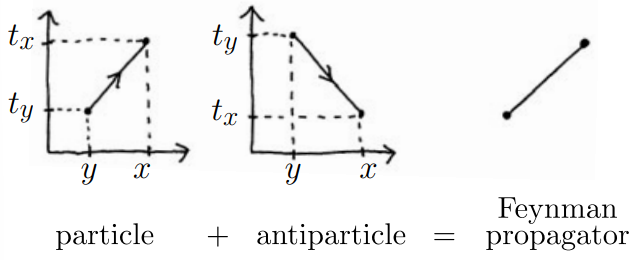
\includegraphics[width=0.6\linewidth]{Immagini/rappr. grafica prop. feynman.png}
    \caption{rappresentazione grafica del propagatore di Feynman vista come somma dei contributi di particella ed antiparticella.}
    \label{fig: rappr. grafica prop. feynman}
\end{figure}

La discussione fatta per i campi scalari carichi può chiaramente essere ripetuta per il caso più semplice dei campi scalari neutri dati da \eqref{eq: campo scalare quantizzato}, in tal caso il propagatore di Feynman è semplicemente 
\begin{equation}
    \Delta(x,y) = \mybrakett{0}{T[\hatphi(x)\hatphi(y)]}{0},
\end{equation}
la cui espressione esplicita è la medesima trovata in \eqref{eq: propagatore libero campo scalare carico (Theta)}.

\subsubsection{Causalità}
Considerando per semplicità il caso dei campi scalari neutri, l'ampiezza di probabilità che una particella si propaghi da un punto $y^\mu$ dello spaziotempo ad un altro $x^\mu$ è, come detto prima, data dall'integrale Lorentz invariante
\begin{equation}
\label{eq: propagatore libero campo scalare carico parziale}
    D(x - y) = \int\frac{d^3k}{(2\pi)^3}\frac{1}{(2\omega_k)}e^{-ik_\mu(x^\mu - y^\mu)}.
\end{equation}
Ci si concentra ora sul risolvere questo integrale per particolari valori della differenza $x^\mu - y^\mu$. Si supponga quindi che la differenza $x^\mu - y^\mu$ sia puramente temporale, ossia che $x^0 - y^0 = t$ e che $\vx -\vy = \bm{0}$, in questo caso si ha
\begin{equation}
    \begin{split}
        D(x - y) &= \frac{4\pi}{(2\pi)^{3}}\int_\R dk\,\frac{p^2}{2\sqrt{p^2 + m^2}}e^{-i\sqrt{p^2 + m^2}t} \\
        &=\frac{1}{4\pi^2}\int_m^\infty dE\, \sqrt{E^2 - m^2}e^{-iEt} \\
        &\overset{t\to\infty}{\simeq} e^{-imt}.
    \end{split}
\end{equation}
Ora si consideri invece che la distanza spaziotemporale $x^\mu - y^\mu$ sia puramente spaziale, ossia che $x^0 - y^0 = 0$ e che $\vx -\vy = \bm{r}$, in questo caso si ha
\begin{equation}
    \begin{split}
        D(x - y) &= \int\frac{d^3k}{(2\pi)^3}\frac{1}{2\omega_k}e^{ik_ir^i} \\
        &= \frac{2\pi}{(2\pi)^3}\int_0^\infty dk\,\frac{p^2}{2\omega_k}\frac{e^{i|\vp||\vr|} - e^{-i|\vp||\vr|}}{i|\vp||\vr|} \\ 
        &= \frac{-i}{2(2\pi)^2|\vr|}\int_\R \frac{|\vp|e^{i|\vp||\vr|}}{\sqrt{p^2 + m^2}}\\
        &=\frac{1}{4\pi^2|\vr|}\int_m^\infty d\rho\,\frac{\rho e^{-\rho|\vr|}}{\sqrt{\rho^2 - m^2}} \\
        &\overset{r\to\infty}{\simeq} e^{-mr},
    \end{split}
\end{equation}
dove, considerando l'integrando come una funzione complessa di $|\vp|$, si è definito $\rho = -i|\vp|$ e si è valutato l'integrale modificando il cammino di integrazione a causa dei poli in $\pm im$ scegliendo di chiuderlo nel semipiano immaginario positivo. Questi due risultati affermano che l'ampiezza di probabilità fuori dal cono luce decresce esponenzialmente ma non è identicamente nulla. Tuttavia, per discutere la causalità si dovrebbe in realtà chiedersi non se le particelle possono propagarsi seguendo specifici intervalli, ma se una misura effettuata in un punto dello spaziotempo può influenzare una misura effettuata in un altro punto separato dal primo da una distanza di tipo spazio. L'elemento più semplice che si può misurare è proprio il campo $\hatphi(x)$, quindi si considera il commutatore $\comm{\hatphi(x)}{\hatphi(y)}$: se questo si annulla, allora una misura non può influenzarne un'altra. Chiaramente, dalle condizioni \eqref{eq: regole di commutazione campo scalare quantizzato} è già noto che il commutatore in questione si annulli per $x^0  = y^0$, si svolge quindi il calcolo più generale
\begin{equation}
    \begin{split}
        \comm{\hatphi(x)}{\hatphi(y)} &= \iint\frac{d^3k\,d^3k'}{(2\pi)^{3}(2\omega_k)^{1/2}(2\omega_{k'})^{1/2}}\times \\
        &\times\comm{\hata_k e^{-ik_\mu x^\mu} + \hataT_k e^{ik_\mu x^\mu}}{\hata_{k'} e^{ik'_\mu y^\mu} + \hata_{k'} e^{ik'_\mu y^\mu}} \\
        &= \int\frac{d^3k}{(2\pi)^3}\frac{1}{2\omega_k}(e^{-ik_\mu(x^\mu - y^\mu)} - e^{ik_\mu(x^\mu - y^\mu)}) \\
        &= D(x - y) - D(y - x),
    \end{split}
\end{equation}
dove si sono usate le regole di commutazione \eqref{eq: regole commutazione operatori a campo scalare}. Quando l'intervallo è di tipo spazio per cui $(x^\mu - y^\mu)^2 < 0$ è possibile effettuare una trasformazione di Lorentz sul secondo termine, dato che ogni termine è Lorentz invariante in modo indipendente, passando da $(x^\mu - y^\mu)\to-(x^\mu - y^\mu)$. In questo modo, la differenza $D(x - y) - D(y - x)$ si annulla e la causalità è conservata. Si osservi inoltre che se $(x^\mu - y^\mu)^2 > 0$ non esiste una trasformazione di Lorentz continua che permetta il passaggio $(x^\mu - y^\mu)\to-(x^\mu - y^\mu)$, in questo caso l'ampiezza di probabilità è diversa da zero, in particolare per $\vx - \vy = \bm{0}$ è circa $(e^{-imt} - e^{imt})$. Dunque, si conclude che nessuna misura in una teoria di campo scalare può influenzare un'altra misura fuori dal cono luce. 

Un discorso analogo può essere fatto nel caso di campi scalari carichi, dove il campo $\hatphi(x)$ genera particelle cariche positivamente e distrugge particelle caricate negativamente, mentre il suo aggiunto $\hatphid(x)$ effettua le operazioni opposte. Quindi, il commutatore $\comm{\hatphi(x)}{\hatphid(y)}$ avrà contributi non nulli che si devono però annullare fuori dal cono luce in modo da preservare la causalità. I due contributi sono interpretati nel medesimo modo in cui si sono interpretati $D(x - y)$ e $D(y - x)$, solo con l'aggiunta della carica: il primo rappresenta la propagazione di una particella carica negativamente da $y^\mu$ a $x^\mu$, mentre il secondo quella di una carica positivamente  da $x^\mu$ a $y^\mu$. Affinché questi due processi generino ampiezze di probabilità opposte è necessario che entrambe le particelle esistano e che abbiano la medesima massa. In Teoria dei campi quindi, la causalità richiede che per ogni particella esista una corrispondente antiparticella avente la medesima massa e numeri quantici opposti, in questo caso la carica elettrica. Per un campo scalare neutro, ogni particella è l'antiparticella di se stessa.

\section{Propagatore di Feynman}
Si vuole ora determinare l'espressione esplicita del propagatore di Feynman ricavato nell'equazione \eqref{eq: propagatore libero campo scalare carico (Theta)}. In realtà, convenzionalmente si pone $\Delta(x,y) = i\Delta_F(x,y)$, dove $\Delta_F(x,y)$ prende effettivamente il nome di propagatore di Feynman. Quindi, prima di tutto si pone $z^\mu \equiv x^\mu - y^\mu$ e si scrive il propagatore di Feynman usando la normalizzazione Lorentz invariante
\begin{equation}
\label{eq: propagatore di Feynman norm. Lorentz invariante}
    i\Delta_F(x,y) = \int \frac{d^4p}{(2\pi)^3}\,\Theta(p_0)\delta(p^2 - m^2)[\Theta(z^0)e^{-ip_\mu z^\mu} + \Theta(-z^0)e^{ip_\mu z^\mu}]
\end{equation}
e si osserva come questa sia una definizione a tratti a causa delle Theta di Heaviside $\Theta(p_0)$ e $\Theta(\pm z^0)$. Per ``rimuovere'' questi contributi si considera l'espressione integrale della Theta ricavabile tramite il teorema di Cauchy
\begin{equation}
\label{eq: espressione integrale Theta Heaviside}
    \Theta(z^0) = \lim_{\epsilon\to0^+}\frac{1}{2i\pi}\int_\R d\tau\,\frac{e^{i\tau z^0}}{\tau - i\epsilon}.
\end{equation}
Per semplicità nel seguito si trascurano i termini $\mathcal{O}(\epsilon^2)$ e si sottintende il limite per $\epsilon\to0^+$. Sostituendo l'espressione \eqref{eq: espressione integrale Theta Heaviside} nella \eqref{eq: propagatore di Feynman norm. Lorentz invariante} si ottiene
\begin{equation}
    \begin{split}
        i\Delta_F(x,y) &= \int \frac{d^4p}{i(2\pi)^4}\int_\R d\tau\,\Theta(p_0)\delta(p^2 - m^2) \\
        &\times\bigg[\frac{e^{-i(p_\mu z^\mu - \tau z^0)}}{\tau - i\epsilon} + \frac{e^{i(p_\mu z^\mu - \tau z^0)}}{\tau - i\epsilon}\bigg].
    \end{split}
\end{equation}
Considerando il secondo termine nella parentesi quadra, si effettua un cambio di variabili $p_\mu \to -p_\mu$ e $\tau \to -\tau$ in modo da avere
\begin{equation}
    \Theta(p_0) \to \Theta(-p_0),\quad 
        \dfrac{e^{i(p_\mu z^\mu - \tau z^0)}}{\tau - i\epsilon} \to \dfrac{e^{-i(p_0z^0 - p_i z^i - \tau z^0)}}{-\tau - i\epsilon} \equiv \dfrac{e^{-ip'_\mu z^\mu}}{-\tau - i\epsilon},
\end{equation}
dove si è definito il quadrimpulso $p_\mu' = (p'_0,p'_i) = (p_0 - \tau,p_i)$, il quale si deve notare non soddisfa l'equazione di mass-shell in quanto ora $\vp'^{\,2} + m^2 = \omega_{p'}^2$. Con questa definizione di $p_\mu'$ si possono anche riscrivere
\begin{align}
    \delta(p^2 - m^2) &= \delta(p_0^2 - p_i^2 - m^2) \notag\\
    &= \delta((p'_0 + \tau)^2 - p_i'^{\,2} - m^2) \\
    &= \frac{\delta(p'_0 + \tau + \omega_{p'})}{2\omega_{p'}} + \frac{\delta(p'_0 + \tau - \omega_{p'})}{2\omega_{p'}}, \notag\\
    \Theta(\pm p_0) &= \Theta(\pm p_0' \pm \tau).
\end{align}
Dunque, si ottiene
\begin{equation}
    \begin{split}
        i\Delta_F(x,y) &= \int\frac{d^4p'}{i(2\pi)^4}\int_\R d\tau\,e^{-ip_\mu'z^\mu}\bigg[\frac{\Theta(p_0' + \tau)}{\tau - i\epsilon} + \frac{\Theta(-p_0' - \tau)}{-\tau - i\epsilon}\bigg]\times \\
        &\times\bigg[\frac{\delta(p'_0 + \tau + \omega_{p'})}{2\omega_{p'}} + \frac{\delta(p'_0 + \tau - \omega_{p'})}{2\omega_{p'}}\bigg] \\
        &= \int\frac{d^4p'}{i(2\pi)^4}\int_\R d\tau\,e^{-ip_\mu'z^\mu}\bigg[\frac{\delta(p'_0 + \tau + \omega_{p'})}{2\omega_{p'}}\frac{\Theta(-p_0' - \tau)}{-\tau - i\epsilon}+ \\
        &+ \frac{\delta(p'_0 + \tau - \omega_{p'})}{2\omega_{p'}}\frac{\Theta(p_0' + \tau)}{\tau - i\epsilon}\bigg].
    \end{split}
\end{equation}
Adesso, sfruttando le delta di Dirac e integrando su $d\tau$ si ha
\begin{equation}
    \begin{split}
        i\Delta_F(x,y) &= \int\frac{d^4p'}{i(2\pi)^4}\frac{e^{-ip_\mu'z^\mu}}{2\omega_{p'}}\bigg(\frac{1}{p_0' + \omega_{p'} - i\epsilon} + \frac{1}{-p_0' + \omega_{p'} - i\epsilon}\bigg) \\
        &= \int\frac{d^4p'}{i(2\pi)^4}\frac{e^{-ip_\mu'z^\mu}}{2\omega_{p'}}\frac{2\omega_{p'} - 2i\epsilon}{(\omega_p' - i\epsilon)^2 - (p_0')^2} \\
        &= \int\frac{d^4p'}{i(2\pi)^4}\frac{e^{-ip_\mu'z^\mu}}{\omega_{p'}^2 - (p_0')^2},
    \end{split}
\end{equation}
che considerando la relazione $\omega_{p'}^2 - (p_0')^2 = p_i^2 + m^2 - (p_0')^2 = m^2 - p'^{\,2}$ e scalando $-2i\epsilon\omega_{p'}\to -i\epsilon$ permette di ottenere un'espressione per il propagatore di Feynman nello spazio delle coordinate
\begin{equation}
\label{eq: propagatore libero campo scalare carico}
    \Delta_F(x,y) = \int\frac{d^4p}{(2\pi)^4}\frac{e^{-ip_\mu'z^\mu}}{p^2 - m^2 + i\epsilon}.
\end{equation}
Nello spazio degli impulsi invece, tramite una trasformata di Fourier, il propagatore di Feynman assume la forma
\begin{equation}
\label{eq. propagatore libero campo scalare carico (spazio impulsi)}
    \tilde{\Delta}_F(p) = \frac{1}{p^2 - m^2 + i\epsilon}.
\end{equation}
In entrambi i risultati \eqref{eq: propagatore libero campo scalare carico} e \eqref{eq. propagatore libero campo scalare carico (spazio impulsi)}, il termine a denominatore $i\epsilon$ assume il ruolo fondamentale di preservare la causalità e dalla rappresentazione integrale della Theta di Heaviside \eqref{eq: espressione integrale Theta Heaviside}, facendo attenzione a considerare il corretto contorno di integrazione dal punto di vista fisico tra le quattro scelte matematicamente equivalenti possibili.

Si può infine verificare che il propagatore in \eqref{eq: propagatore libero campo scalare carico} è la funzione di Green dell'operatore di Klein-Gordon $(\square + m^2)$, infatti
\begin{equation}
    (\square + m^2)\Delta_F(x,y) = \int\frac{d^4p}{(2\pi)^4}\frac{-p^2 + m^2}{p^2 - m^2 + i\epsilon}e^{-p_\mu z^\mu},
\end{equation}
considerando poi che il fattore $i\epsilon$ può essere mandato a zero grazie al limite sottinteso per $\epsilon\to0^+$ si ha proprio
\begin{equation}
     (\square + m^2)\Delta_F(x,y) = -\int\frac{d^4p}{(2\pi)^4}e^{-p_\mu z^\mu} = -\delta^4(x - y).
\end{equation}
In aggiunta, nel caso dei campi vettoriali, che descrivono particelle come il fotone, si definisce il propagatore come
\begin{equation}
    \Delta(x,y) = \frac{1}{k^2 - i\epsilon}.
\end{equation}
Invece, per il campo spinoriale di Dirac si definisce il propagatore come
\begin{equation}
    iS_F(x,y) = \mybrakett{0}{T[\hatpsi(x)\hatpsib(y)]}{0}
\end{equation}
che, seguendo un processo analogo a quanto fatto per il campo scalare anche se più tortuoso a causa dell'algebra delle matrici $\gamma^\mu$, ha come forma esplicita nello spazio dello coordinate 
\begin{equation}
\label{eq: propagatore campo spinoriale}
    S_F(x,y) = \int\frac{d^4p}{(2\pi)^4}\frac{\slp + m}{p^2 - m^2 + i\epsilon},
\end{equation}
mentre nello spazio degli impulsi risulta essere
\begin{equation}
    \tilde{S}_F(p) = \frac{\slp + m}{p^2 - m^2} = \frac{i}{\slp - m}. 
\end{equation}